% Soubory musí být v kódování, které je nastaveno v příkazu \usepackage[...]{inputenc}

\documentclass[%        Základní nastavení
  %draft,    				  % Testovací překlad
  12pt,       				% Velikost základního písma je 12 bodů
	t,                  % obsah slajdů bude vždy začínat od shora (nebude vertikálně centrovaný)
	aspectratio=1610,   % poměr stran bude 16:10 (všechny projektory v učebnách na Technické 12 Brno),
	                    % další volby jsou 43, 149, 169, 54, 32.
	unicode,						% Záložky a informace budou v kódování unicode
]{beamer}				    	% Dokument třídy 'zpráva', vhodná pro sazbu závěrečných prací s kapitolami
%\usepackage{etex}

\usepackage[utf8]		  % Kódování zdrojových souborů je v UTF-8
	{inputenc}					% Balíček pro nastavení kódování zdrojových souborů
	
\usepackage{graphicx} % Balíček 'graphicx' pro vkládání obrázků
											% Nutné pro vložení logotypů školy a fakulty

\usepackage[          % Balíček 'acronym' pro sazby zkratek a symbolů
	nohyperlinks				% Nebudou tvořeny hypertextové odkazy do seznamu zkratek
]{acronym}						
											% Nutné pro použití prostředí 'acronym' balíčku 'thesis'

%% Balíček hyperref je volán třídou beamer automaticky, proto není třeba následujícího kódu:
%\usepackage[
%	breaklinks=true,		% Hypertextové odkazy mohou obsahovat zalomení řádku
%	hypertexnames=false % Názvy hypertextových odkazů budou tvořeny
%											% nezávisle na názvech TeXu
%]{hyperref}						% Balíček 'hyperref' pro sazbu hypertextových odkazů
%											% Nutné pro použití příkazu 'nastavenipdf' balíčku 'thesis'

\usepackage{cmap} 		% Balíček cmap zajišťuje, že PDF vytvořené `pdflatexem' je
											% plně "prohledávatelné" a "kopírovatelné"

%\usepackage{upgreek}	% Balíček pro sazbu stojatých řeckých písmem
											%% např. stojaté pí: \uppi
											%% např. stojaté mí: \upmu (použitelné třeba v mikrometrech)
											%% pozor, grafická nekompatibilita s fonty typu Computer Modern!

%\usepackage{amsmath} %balíček pro sabu náročnější matematiky

\usepackage{booktabs} % Balíček, který umožňuje v tabulce používat
                      % příkazy \toprule, \midrule, \bottomrule


%%%%%%%%%%%%%%%%%%%%%%%%%%%%%%%%%%%%%%%%%%%%%%%%%%%%%%%%%%%%%%%%%
%%%%%%      Definice informací o dokumentu             %%%%%%%%%%
%%%%%%%%%%%%%%%%%%%%%%%%%%%%%%%%%%%%%%%%%%%%%%%%%%%%%%%%%%%%%%%%%

% V tomto souboru se nastavují téměř veškeré informace, proměnné mezi studenty:
% jméno, název práce, pohlaví atd.
% Tento soubor je SDÍLENÝ mezi textem práce a prezentací k obhajobě -- netřeba něco nastavovat na dvou místech.

\usepackage[
%%% Z následujících voleb jazyka lze použít pouze jednu
  czech-english,		% originální jazyk je čeština, překlad je anglicky (výchozí)
  %english-czech,	% originální jazyk je angličtina, překlad je česky
  %slovak-english,	% originální jazyk je slovenština, překlad je anglicky
  %english-slovak,	% originální jazyk je angličtina, překlad je slovensky
%
%%% Z následujících voleb typu práce lze použít pouze jednu
  semestral,		  % semestrální práce (nesází se abstrakty, prohlášení, poděkování) (výchozí)
  %bachelor,			%	bakalářská práce
  %master,			  % diplomová práce
  %treatise,			% pojednání o disertační práci
  %doctoral,			% disertační práce
%
%%% Z následujících voleb zarovnání objektů lze použít pouze jednu
%  left,				  % rovnice a popisky plovoucích objektů budou zarovnány vlevo
	center,			    % rovnice a popisky plovoucích objektů budou zarovnány na střed (vychozi)
%
]{thesis}   % Balíček pro sazbu studentských prací

\usepackage{microtype}

%%% Jméno a příjmení autora ve tvaru
%  [tituly před jménem]{Křestní}{Příjmení}[tituly za jménem]
% Pokud osoba nemá titul před/za jménem, smažte celý řetězec '[...]'
\author[Bc.]{Renata}{Zemanová}

%%% Identifikační číslo autora (VUT ID)
\butid{211251}

%%% Pohlaví autora/autorky
% (nepoužije se ve variantě english-czech ani english-slovak)
% Číselná hodnota: 1...žena, 0...muž
\gender{1}

%%% Jméno a příjmení vedoucího/školitele včetně titulů
%  [tituly před jménem]{Křestní}{Příjmení}[tituly za jménem]
% Pokud osoba nemá titul před/za jménem, smažte celý řetězec '[...]'
\advisor[doc.\ Ing.]{Pavel}{Šteffan}[Ph.D.]

%%% Jméno a příjmení oponenta včetně titulů
%  [tituly před jménem]{Křestní}{Příjmení}[tituly za jménem]
% Pokud osoba nemá titul před/za jménem, smažte celý řetězec '[...]'
% Nastavení oponenta se uplatní pouze v prezentaci k obhajobě;
% v případě, že nechcete, aby se na titulním snímku prezentace zobrazoval oponent, pouze příkaz zakomentujte;
% u obhajoby semestrální práce se oponent nezobrazuje (jelikož neexistuje)
% U dizertační práce jsou typicky dva až tři oponenti. Pokud je chcete mít na titulním slajdu, prosím ručně odkomentujte a upravte jejich jména v definici "VUT title page" v souboru thesis.sty.
\opponent[doc.\ Mgr.]{Křestní}{Příjmení}[Ph.D.]

%%% Název práce
%  Parametr ve složených závorkách {} je název v originálním jazyce,
%  parametr v hranatých závorkách [] je překlad (podle toho jaký je originální jazyk).
%  V případě, že název Vaší práce je dlouhý a nevleze se celý do zápatí prezentace, použijte příkaz
%  \def\insertshorttitle{Zkác.\ náz.\ práce}
%  kde jako parametr vyplníte zkrácený název. Pokud nechcete zkracovat název, budete muset předefinovat,
%  jak se vytváří patička slidu. Viz odkaz: https://bit.ly/3EJTp5A
\title[Traffic light - technological equivalent of a streamer]{Semafor - technologický ekvivalent fáborku}

%%% Označení oboru studia
%  Parametr ve složených závorkách {} je název oboru v originálním jazyce,
%  parametr v hranatých závorkách [] je překlad
\specialization[Microelectronics]{Mikroelektronika}

%%% Označení ústavu
%  Parametr ve složených závorkách {} je název ústavu v originálním jazyce,
%  parametr v hranatých závorkách [] je překlad
%\department[Department of Control and Instrumentation]{Ústav automatizace a měřicí techniky}
%\department[Department of Biomedical Engineering]{Ústav biomedicínského inženýrství}
%\department[Department of Electrical Power Engineering]{Ústav elektroenergetiky}
%\department[Department of Electrical and Electronic Technology]{Ústav elektrotechnologie}
%\department[Department of Physics]{Ústav fyziky}
%\department[Department of Foreign Languages]{Ústav jazyků}
%\department[Department of Mathematics]{Ústav matematiky}
\department[Department of Microelectronics]{Ústav mikroelektroniky}
%\department[Department of Radio Electronics]{Ústav radioelektroniky}
%\department[Department of Theoretical and Experimental Electrical Engineering]{Ústav teoretické a experimentální elektrotechniky}
%\department[Department of Telecommunications]{Ústav telekomunikací}
%\department[Department of Power Electrical and Electronic Engineering]{Ústav výkonové elektrotechniky a elektroniky}

%%% Označení fakulty
%  Parametr ve složených závorkách {} je název fakulty v originálním jazyce,
%  parametr v hranatých závorkách [] je překlad
%\faculty[Faculty of Architecture]{Fakulta architektury}
\faculty[Faculty of Electrical Engineering and~Communication]{Fakulta elektrotechniky a~komunikačních technologií}
%\faculty[Faculty of Chemistry]{Fakulta chemická}
%\faculty[Faculty of Information Technology]{Fakulta informačních technologií}
%\faculty[Faculty of Business and Management]{Fakulta podnikatelská}
%\faculty[Faculty of Civil Engineering]{Fakulta stavební}
%\faculty[Faculty of Mechanical Engineering]{Fakulta strojního inženýrství}
%\faculty[Faculty of Fine Arts]{Fakulta výtvarných umění}
%
%Nastavení logotypu (v hranatych zavorkach zkracene logo, ve slozenych plne):
\facultylogo[logo/FEKT_zkratka_barevne_PANTONE_CZ]{logo/UTKO_color_PANTONE_CZ}

%%% Rok odevzdání práce
\graduateyear{2023}
%%% Akademický rok odevzdání práce
\academicyear{2022/23}

%%% Datum obhajoby (uplatní se pouze v prezentaci k obhajobě)
\date{11.\,01.\,2023} 

%%% Místo obhajoby
% Na titulních stránkách bude automaticky vysázeno VELKÝMI písmeny (pokud tyto stránky sází šablona)
\city{Brno}

%%% Abstrakt
\abstract[%
The goal of this semestral thesis is to design device called Traffic light, which serves as an assistant in outdoor games and for education
purposes. The design focuses on safety, simplicity and low cost. 

This thesis deals with the selection and design of the overall electronics contained in the Traffic light. Emphasis is placed on the selection 
of the light signaling, wireless module and microcontroller.
]{%
Cílem práce je navrhnout elektronické zařízení Semafor, který slouží jako pomocník při outdoorových hrách a pro edukační účely. 
Při návrhu je kladen důraz na bezpečnost, jednoduchost a nízkou cenu. 

Tato práce se zabývá výběrem a návrhem celkové elektroniky, kterou Semafor obsahuje. Je kladen důraz na výběr světelné signalizace, 
bezdrátového modulu a mikrokontroléru. 
}

%%% Klíčová slova
\keywrds[%
Traffic light, microcontroller, programmable LED WS2812C, batteries LiFePO4, LoRa module, capacitive touch buttons
]{%
Semafor, mikrokontrolér, programovatelné LED WS2812C, baterie LiFePO4, LoRa modul, kapacitní dotyková tlačítka
}

%%% Poděkování
\acknowledgement{%
Ráda bych poděkovala vedoucímu diplomové práce panu doc. Ing.~Pavlovi Šteffanovi, Ph.D.\ za odborné vedení,
konzultace, podnětné návrhy k~práci a zapůjčení testovacího hardwaru. Dále také děkuji RNDr. Janovi Mrázkovi 
za podnětné rady při návrhu elektroniky. 
}%      % v tomto souboru doplňte údaje o sobě, o názvu práce...
                       % (tento soubor je sdílený s textem práce)

%%%%%%%%%%%%%%%%%%%%%%%%%%%%%%%%%%%%%%%%%%%%%%%%%%%%%%%%%%%%%%%%%%%%%%%%

%%%%%%%%%%%%%%%%%%%%%%%%%%%%%%%%%%%%%%%%%%%%%%%%%%%%%%%%%%%%%%%%%%%%%%%%
%%%%%%     Nastavení polí ve Vlastnostech dokumentu PDF      %%%%%%%%%%%
%%%%%%%%%%%%%%%%%%%%%%%%%%%%%%%%%%%%%%%%%%%%%%%%%%%%%%%%%%%%%%%%%%%%%%%%
%% Při vloženém balíčku 'hyperref' lze použít příkaz '\pdfsettings'
\pdfsettings
%  Nastavení polí je možné provést také ručně příkazem:
%\hypersetup{
%  pdftitle={Název studentské práce},    	% Pole 'Document Title'
%  pdfauthor={Autor studenstké práce},   	% Pole 'Author'
%  pdfsubject={Typ práce}, 						  	% Pole 'Subject'
%  pdfkeywords={Klíčová slova}           	% Pole 'Keywords'
%}
\hypersetup{pdfpagemode=FullScreen}       % otevření rovnou v režimu celé obrazovky
%%%%%%%%%%%%%%%%%%%%%%%%%%%%%%%%%%%%%%%%%%%%%%%%%%%%%%%%%%%%%%%%%%%%%%%

\usetheme{VUT} 				% barvy a rozložení prezentace odpovídající VUT FEKT
% alternativně lze použít jiná berevná témata, ale bez záruky. Například: 
%\usetheme{Darmstadt} \usecolortheme{default2}
\logoheader					% vytvoření zkráceného loga VUT FEKT v hlavičce slajdu, nechte odkomentované



\begin{document}

% v případě zakomentování následujícího se zobrazí v pravém dolním rohu slajdů klikatelné navigační symboly 
\disablenavigationsymbols

% titulní snímek, vysazen bez horních, dolních a postranních lišt (volba plain),
% není tak vysazen ani nadpis snímku
\maketitle

%%%%%%%%%%%%%%%%%%%%%%%%%%%%%%%%%%%%%%%%%%%%%%%%%%%%%%%%%%%%%%%%%%%%%%%
% 1. snímek s cíli (zadaním) práce
\begin{frame} 
	\frametitle{Základní informace}
	\begin{columns}[T] 								% prostředí sloupce s umístěním nahoře
		\begin{column}{0.5\textwidth}		% první sloupec
			K čemu slouží Univerzální modul?
			\begin{itemize}
				\item Outdoorová aplikace
				\item Edukační účely, táborové hry
				\item Zástupná funkce organizátora
				\item Dotykové senzory
				\item Světelné a zvukové signalizace
			\end{itemize}
		\end{column}
		%
		\begin{column}{0.5\textwidth}		% druhý sloupec
				Požadavky
					\begin{itemize}
						\item Kompaktnost
						\item Bezpečnost
						\item Široké využití
						\item Voděodolnost
						\item Nízká cena
						\item Jednoduchost
						\item Bezdrátová konfigurovatelnost
					\end{itemize}
				%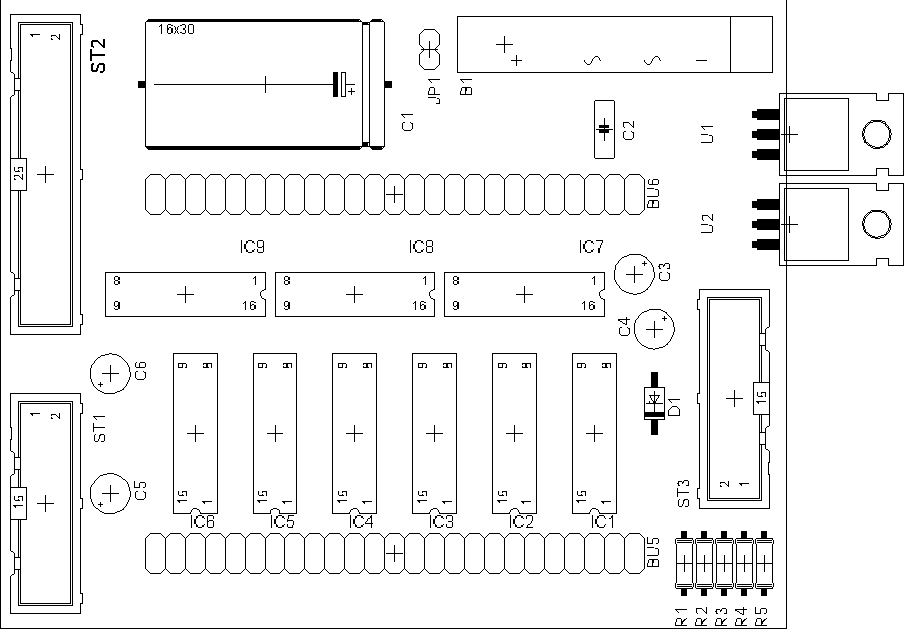
\includegraphics[width=0.8\columnwidth]{obrazky/soucastky}
				%lze vložit popisek, ale povetšinou je to v prezentaci zbytečné
				%\caption{Popisek obrázku}%
				%\label{obr:ukazka}
		\end{column}
	\end{columns}	
\end{frame}

\begin{frame} 
	\frametitle{Cíle práce}

	\begin{columns}[T] 								% prostředí sloupce s umístěním nahoře
		\begin{column}{0.25\textwidth}		% první sloupec
			\begin{itemize}
				\item Nastudovat
				\item Porovnat
				\item Vybrat
				\item Navrhnout 
				\item Vyrobit a osadit 
				\item Naprogramovat
				\item Vyřešit voděodolnost
		\end{itemize}
		\end{column}
		%
		\begin{column}{0.65\textwidth}		% druhý sloupec
			\begin{figure}%	
				\centering
				\vspace{0.4cm}	              % horizontální mezera
				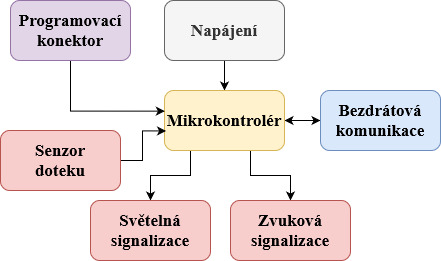
\includegraphics[width=1\columnwidth]{obrazky/zakladni_blokove_schema_prezentace.jpg}
				%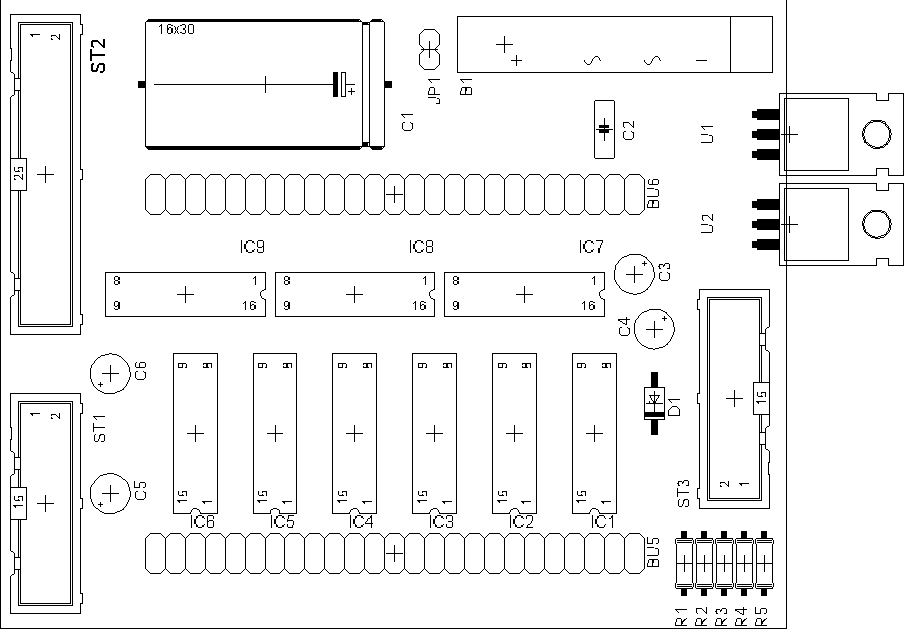
\includegraphics[width=0.8\columnwidth]{obrazky/soucastky}
				%lze vložit popisek, ale povetšinou je to v prezentaci zbytečné
				%\caption{Popisek obrázku}%
				%\label{obr:ukazka}
			\end{figure}
		\end{column}
		\begin{column}{0.1\textwidth}		% druhý sloupec
		\end{column}
	\end{columns}	
		
	\end{frame}


%%%%%%%%%%%%%
\begin{frame} 
	\frametitle{Základní prvky}
	
	\begin{columns}[T] 								% prostředí sloupce s umístěním nahoře
		\begin{column}{0.5\textwidth}		% první sloupec
			%Obrázek znázorňuje model:\\[2ex]
			%
			Bezdrátová konfigurace
			\begin{itemize}
				\item WiFi
				\item Bezlicenční pásmo
				\item Rozšířená 
				\item V každém mobilním telefonu
			\end{itemize}
			Mikrokontrolér
			\begin{itemize}
				\item ESP32-C3-MINI-1
				\item WiFi s anténou 
				\item SPI, UART, $I^2C$, USB
				\item 13 GPIO pinů
			\end{itemize}
		\end{column}
		%
		\begin{column}{0.5\textwidth}		% druhý sloupec
			\begin{itemize}
				\item Napájení
				\begin{itemize}
					\item Baterie LiFePO4
					\item 3 až 3,6 V
					\item Nejbezpečnější
					\item Životnost až 7000 cyklů 
					\item Teplotně stabilní
					\item Nehořlavé, netoxické
				\end{itemize}
				\item Nabíjecí obvod CN3058E
				\item Měření napětí na baterii 
			\end{itemize}
		\end{column}
	\end{columns}											% ukončení prostředí sloupce
\end{frame}

\begin{frame} 
	\frametitle{Komunikace s okolím}
	
	\begin{columns}[T] 								% prostředí sloupce s umístěním nahoře
		\begin{column}{0.5\textwidth}		% první sloupec
			%Obrázek znázorňuje model:\\[2ex]
			Světelná signalizace
			\begin{itemize}
				\item Programovatelné LED WS2812C
				\item Možnost spojení za sebou
				\item Převodník úrovní
				\item Zvyšovač napětí LT1930
			\end{itemize}
			\begin{figure}%	
				\centering	          
				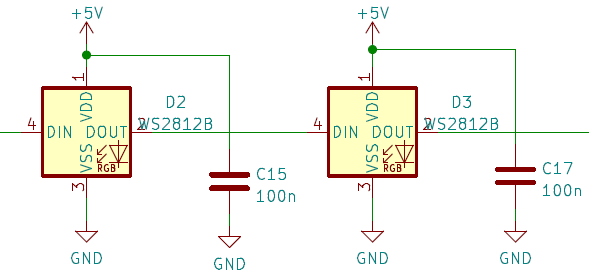
\includegraphics[width=1\columnwidth]{obrazky/WS2812C_prezentace.png}
			\end{figure}
		\end{column}
		%
		\begin{column}{0.5\textwidth}		% druhý sloupec
			Senzory doteku
			\begin{itemize}
				\item Kapacitní tlačítka
				\item Mechanická odolnost
				\item Životnost
				\item Vibrační odezva
				\item Převodník
				\begin{itemize}
					\item Komunikace po $I^2C$
					\item Až 7 tlačítek
				\end{itemize}
			\end{itemize}
		\end{column}
	\end{columns}											% ukončení prostředí sloupce
\end{frame}

\begin{frame} 
	\frametitle{Zapojení elektroniky}
	\begin{figure}%	
		\centering	          
		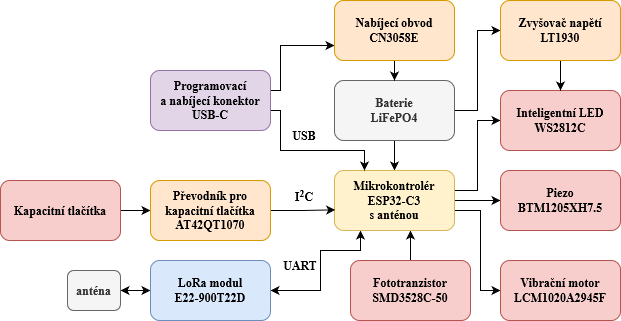
\includegraphics[width=1\columnwidth]{obrazky/blokove_schema_finalni_verze.png}
	\end{figure}
\end{frame}

\begin{frame}
	\frametitle{Výsledné DPS}
	\begin{columns}[T] 	
		\begin{column}{0.5\textwidth}	
			\begin{figure}%	
				\centering	          
				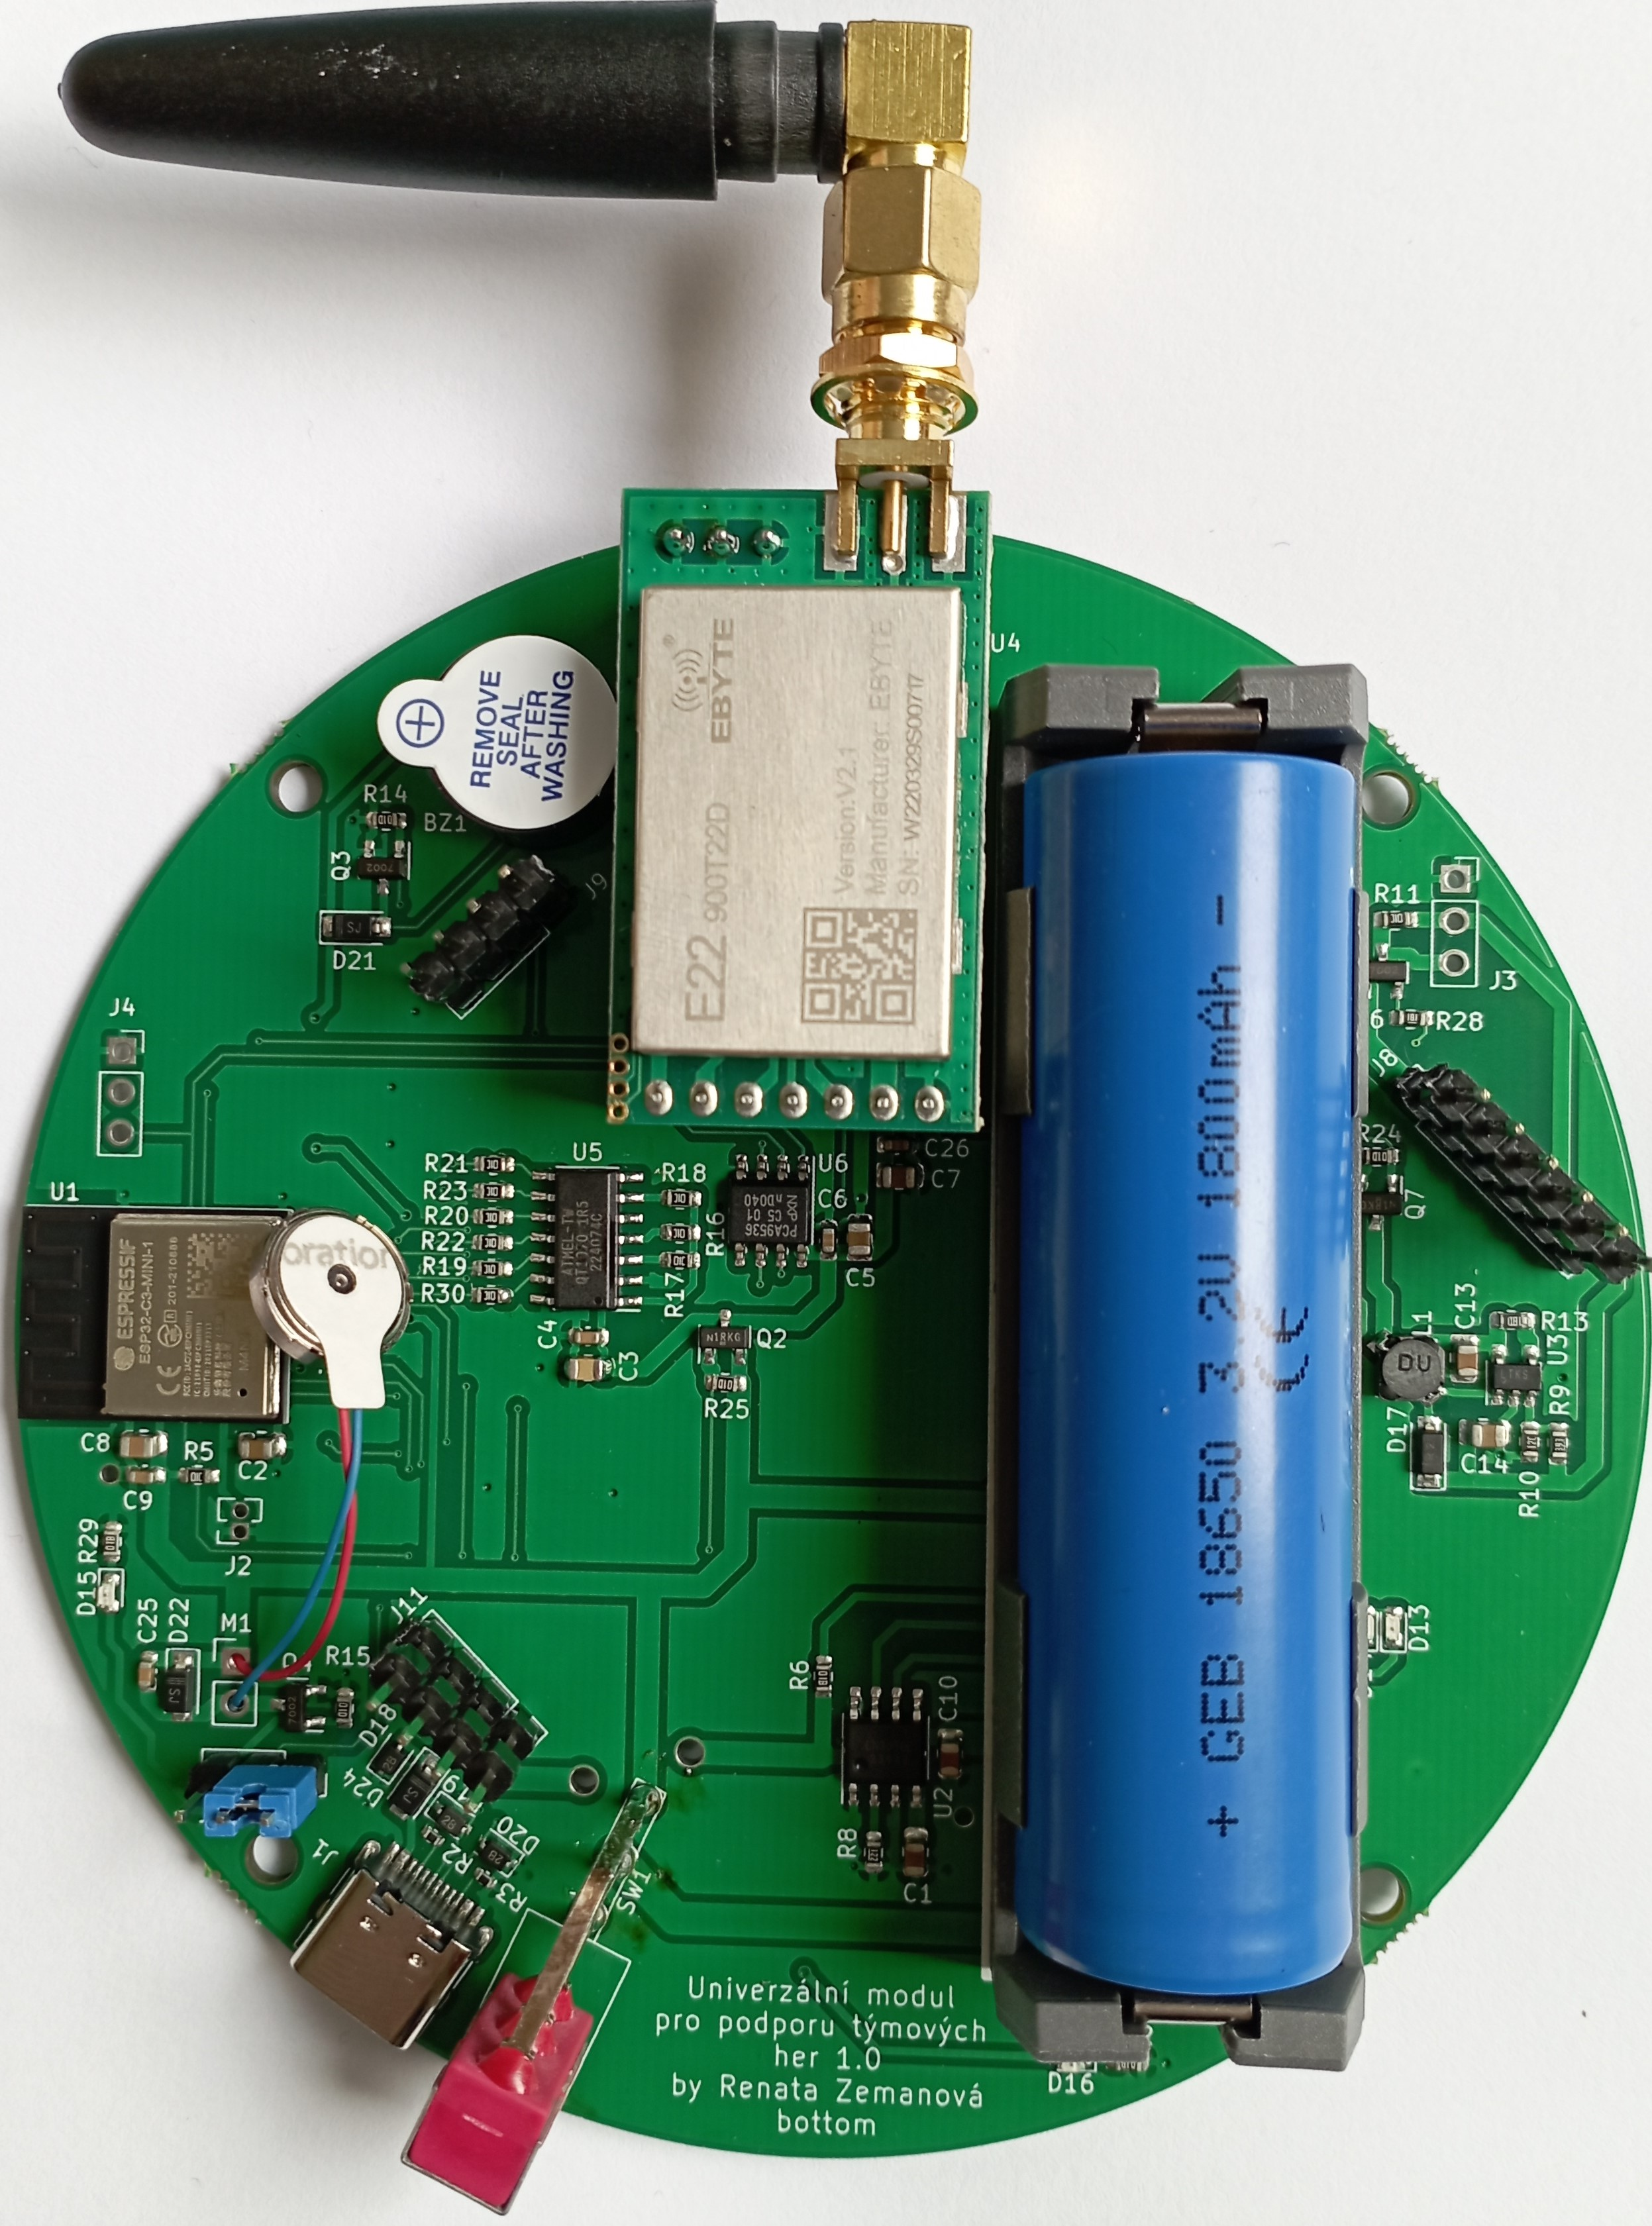
\includegraphics[width=0.7\columnwidth]{obrazky/DPS_final_spodni.jpg}
			\end{figure}
		\end{column}

		\begin{column}{0.5\textwidth}	
			\begin{figure}%	
				\centering	          
				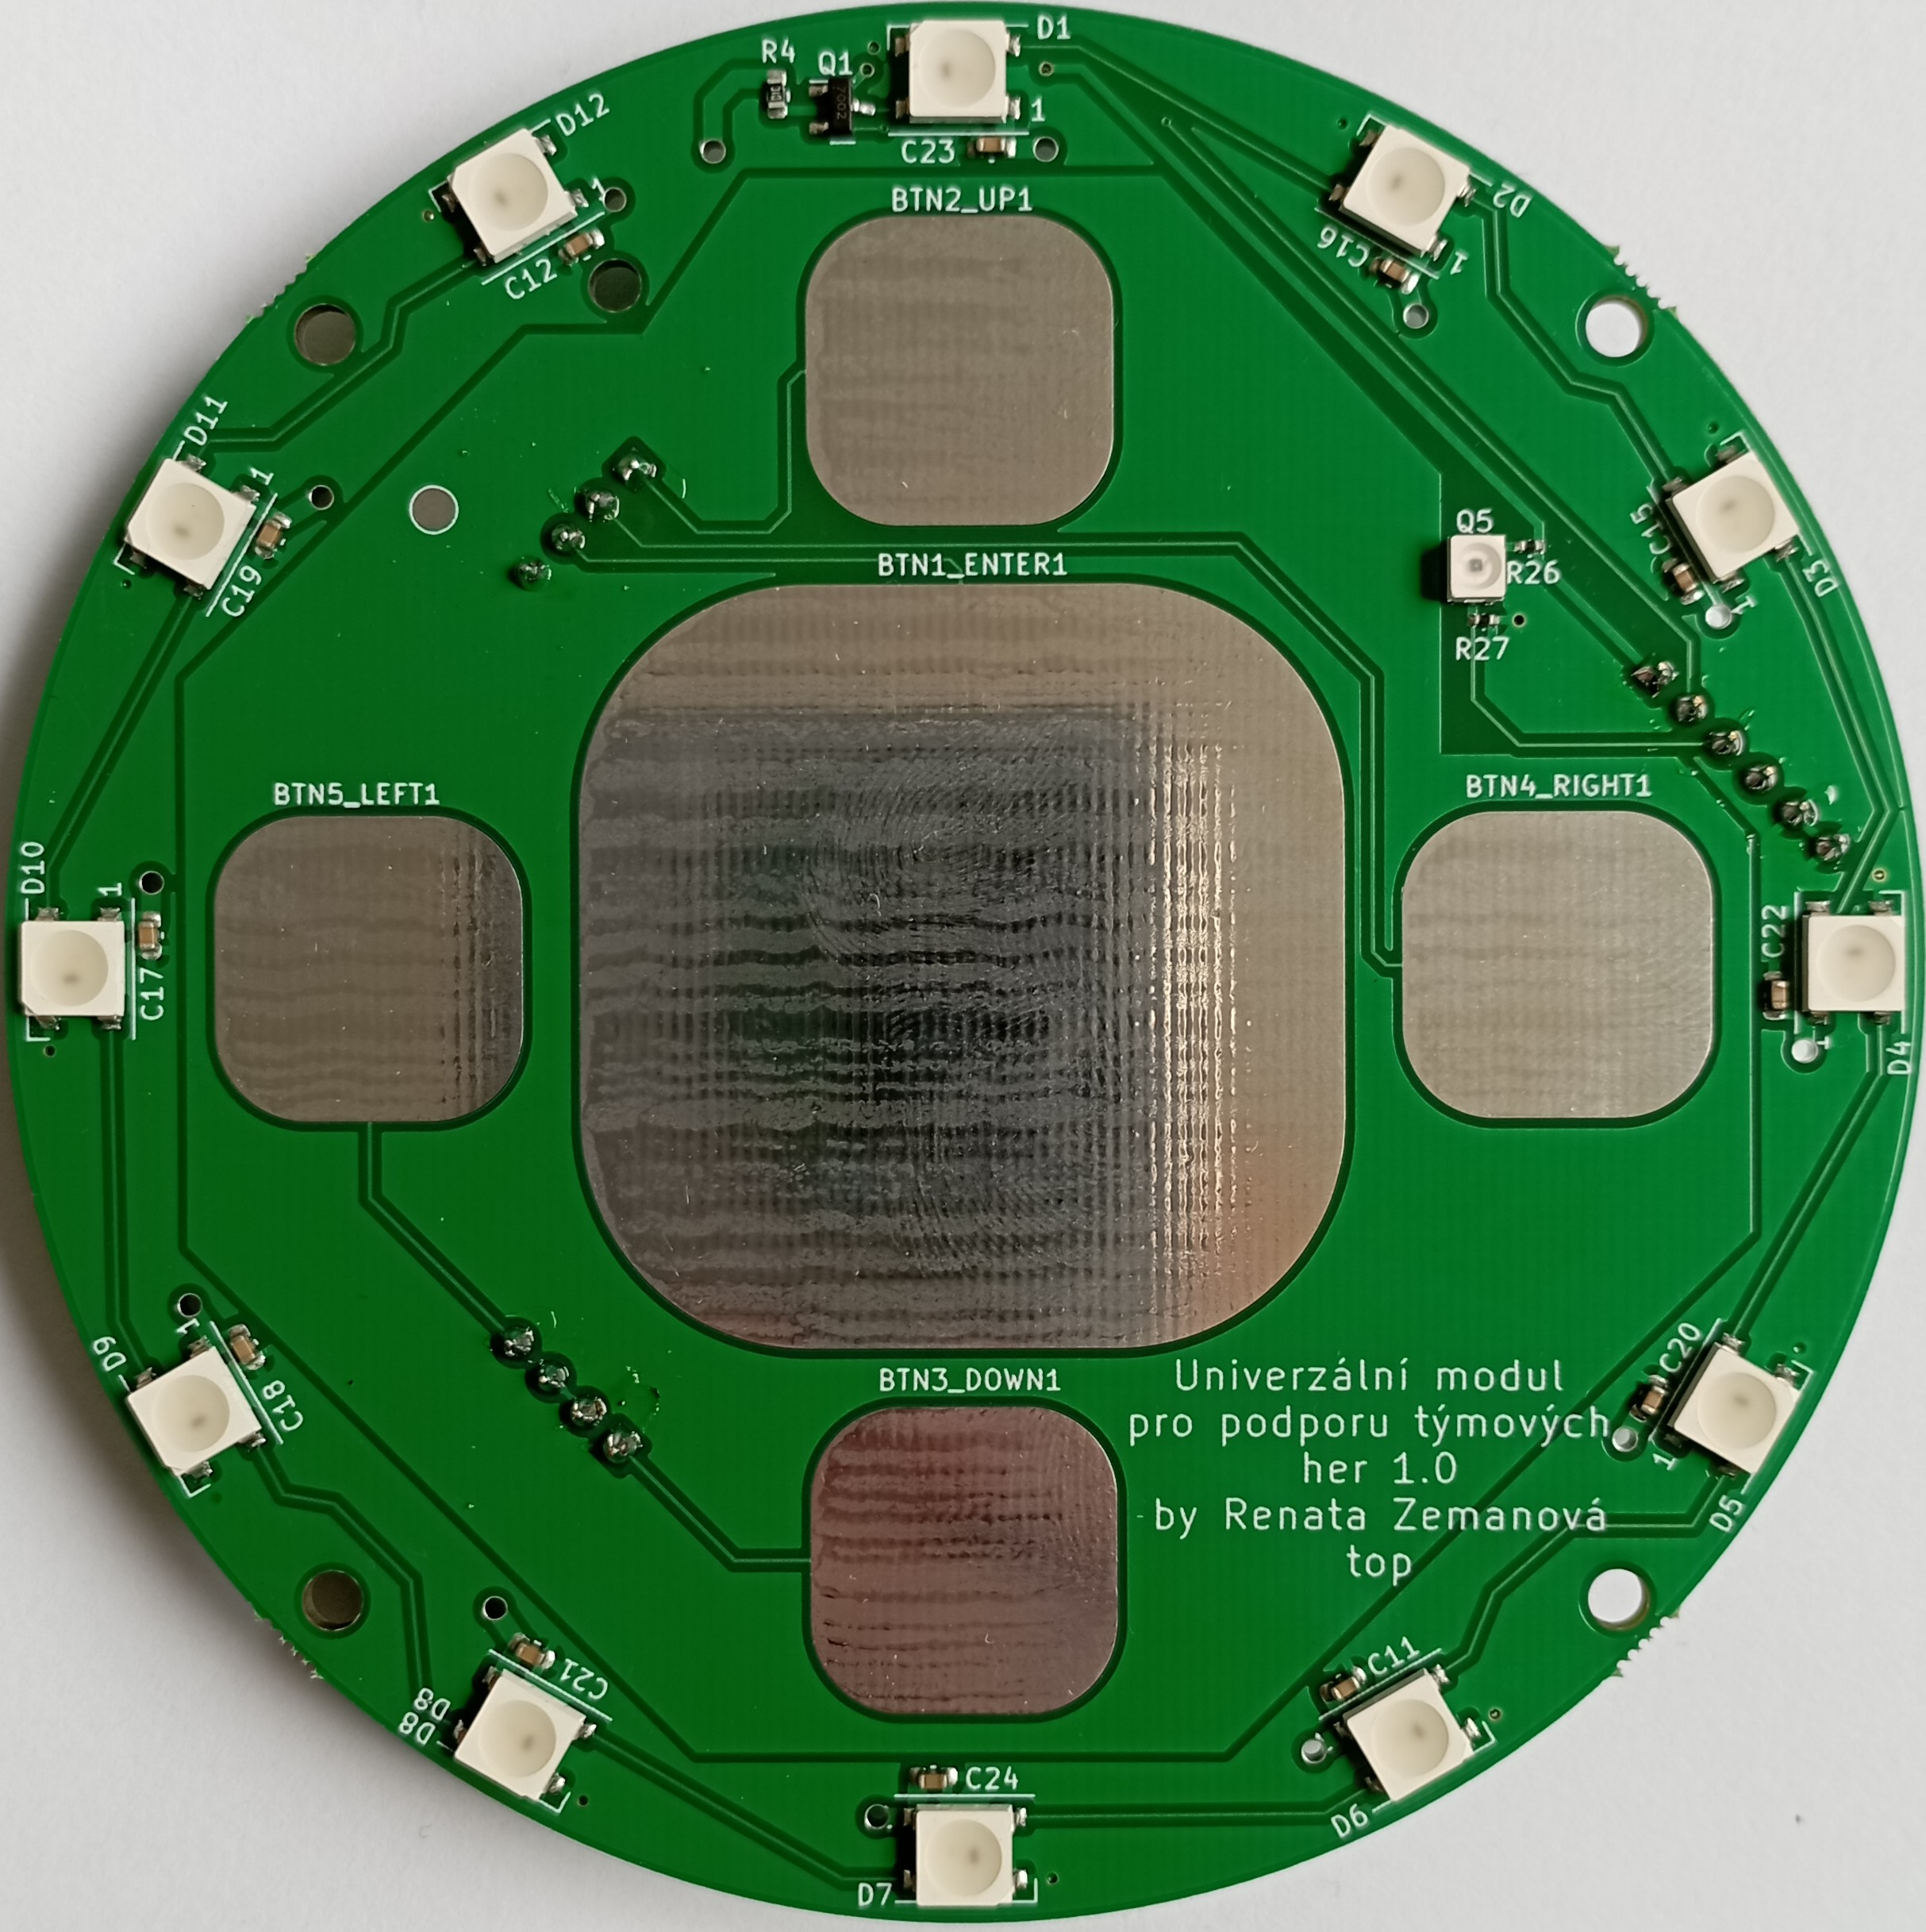
\includegraphics[width=0.9\columnwidth]{obrazky/DPS_final_vrchni.jpg}
			\end{figure}
		\end{column}
	\end{columns}
\end{frame}

\begin{frame}
	\frametitle{Firmware}
	\begin{columns}[T] 	
		\begin{column}{0.35\textwidth}	
			\begin{itemize}	
				\item Práce se senzory 
				\item Měření napětí na baterii
				\item Bezdrátová konfigurace
				\begin{itemize}
					\item WiFi
					\item Jednotlivé módy 
					\item Popisy
					\item Parametry 
				\end{itemize}
			\end{itemize}
		\end{column}

		\begin{column}{0.65\textwidth}	
			\begin{figure}
				\centering	          
				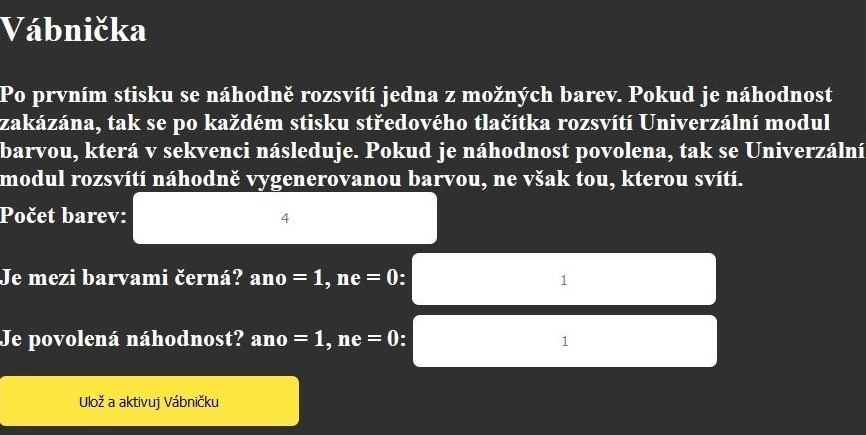
\includegraphics[width=1\columnwidth]{obrazky/konfiguracni_webova_stranka_prezentace.jpg}
			\end{figure}
		\end{column}
	\end{columns}
\end{frame}

\begin{frame}
	\frametitle{Příklad využití}
	\begin{columns}[T] 	
		\begin{column}{0.25\textwidth}	
			\begin{itemize}
				\item 3 módy 
				\item LED, tlačítka 
				\item Vábnička
				\item Klasický semafor
				\item Odpočítávadlo 
			\end{itemize}
		\end{column}

		\begin{column}{0.75\textwidth}	
			\begin{figure}%	
				\centering	          
				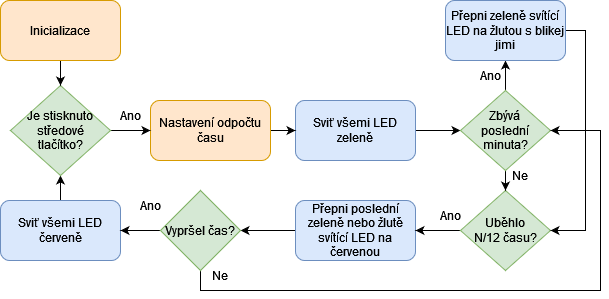
\includegraphics[width=1\columnwidth]{obrazky/Odpocitavani_diagram.png}
			\end{figure}
		\end{column}
	\end{columns}
\end{frame}


\begin{frame}
	\frametitle{Voděodolnost}
	\begin{columns}[T] 	
		\begin{column}{0.3\textwidth}	
			\begin{itemize}
				\item 3D tisk  
				\item Přilepení 
				\item Čirý lak
			\end{itemize}
		\end{column}

		\begin{column}{0.7\textwidth}	
			\begin{figure}%	
				\centering	          
				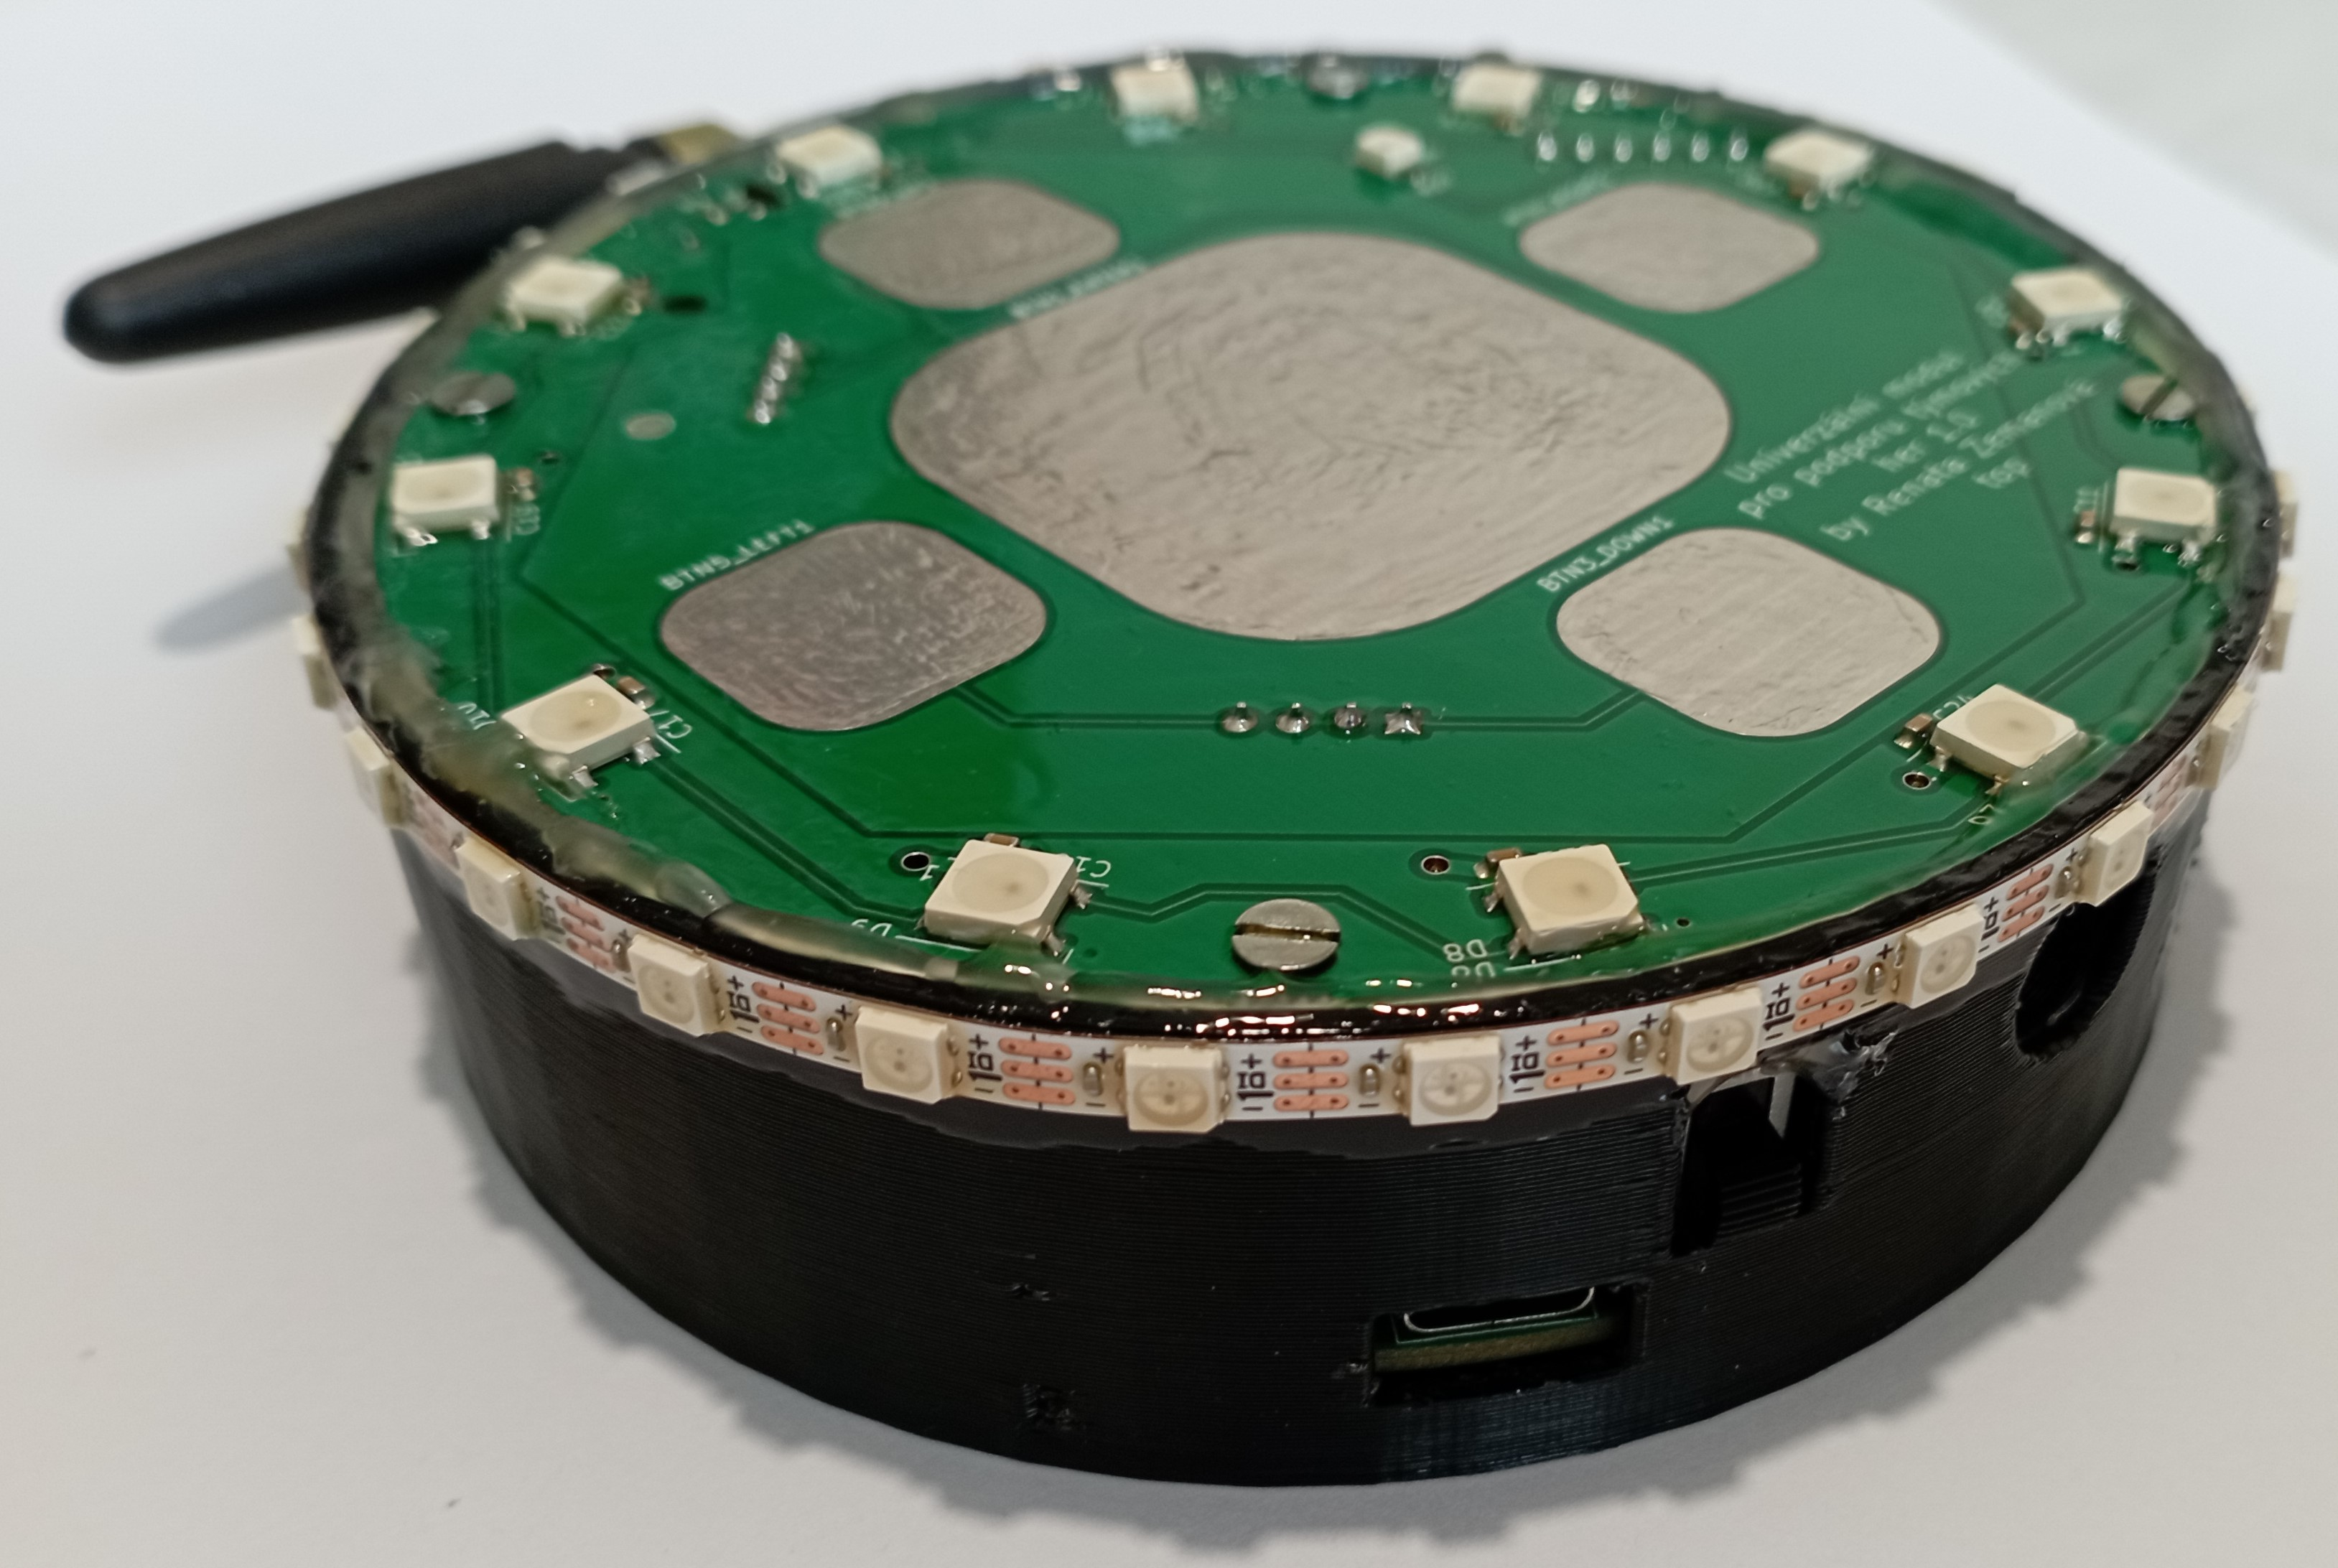
\includegraphics[width=1\columnwidth]{obrazky/v_krabicce_bok.jpg}
			\end{figure}
		\end{column}
	\end{columns}
\end{frame}

%%%%%%%%%%%%%
\begin{frame} 
	\frametitle{Závěr}

	\begin{center}
		\begin{columns}[T] 								% prostředí sloupce s umístěním nahoře
			\begin{column}{0.3\textwidth}		% první sloupec
				\begin{itemize}
					\item Návrh elektroniky
					\item Návrh DPS
					\item Výroba a osazení DPS
					\item Firmware 
					\item Bezdrátová konfigurace
					\item Příklad využití 
					\item Voděodolnost
				\end{itemize}
			\end{column}
			%
			\begin{column}{0.7\textwidth}		% druhý sloupec
				\begin{figure}
					\centering
					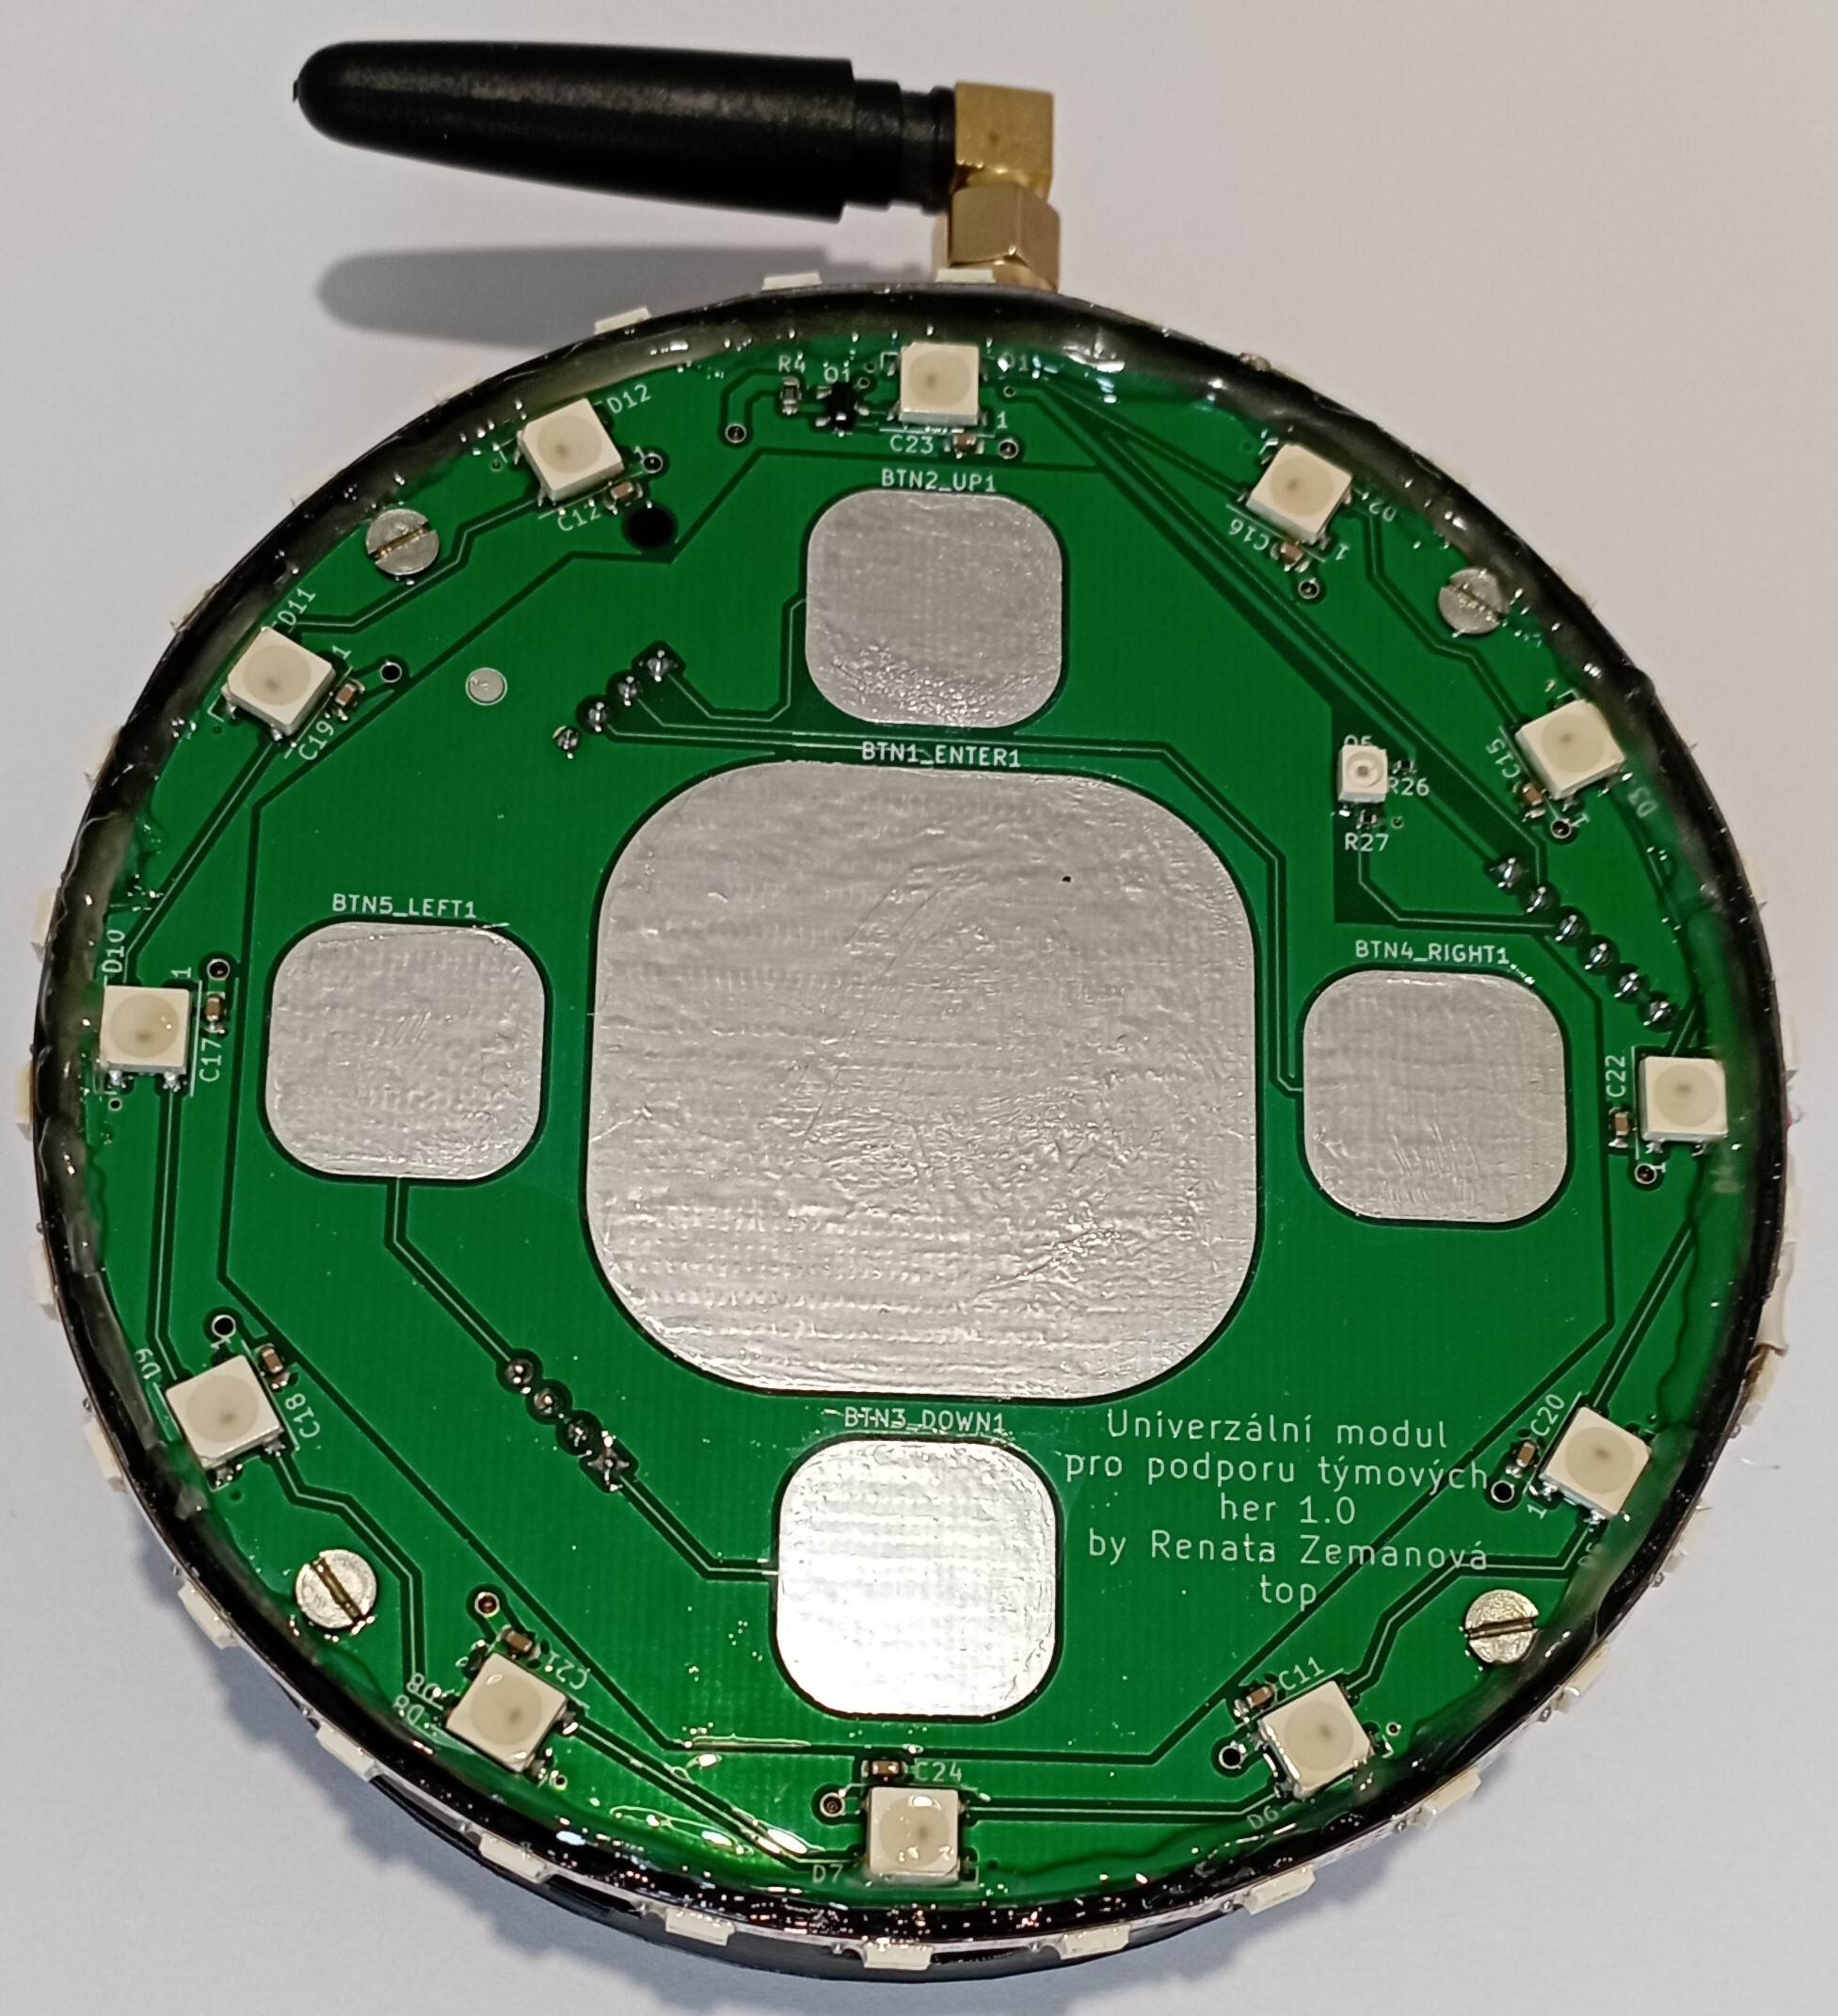
\includegraphics[width=0.65\columnwidth]{obrazky/v_krabicce.jpg}
				\end{figure}
			\end{column}
		\end{columns}	
	\end{center}
	
\end{frame}


% podekovani
\begin{frame}[c] 
% bez nadpisu snímku
	\frametitle{\mbox{ }}
	\begin{center}
		\begin{columns}[T] 								% prostředí sloupce s umístěním nahoře
			\begin{column}{0.3\textwidth}		% první sloupec
				{\Huge Děkuji za pozornost!}
				\vspace{0.5cm}
				\begin{itemize}
					\item Návrh elektroniky
					\item Návrh DPS
					\item Výroba a osazení DPS
					\item Firmware 
					\item Bezdrátová konfigurace
					\item Příklad využití 
					\item Voděodolnost
				\end{itemize}
			\end{column}
			%
			\begin{column}{0.7\textwidth}		% druhý sloupec
				\begin{figure}
					\centering
					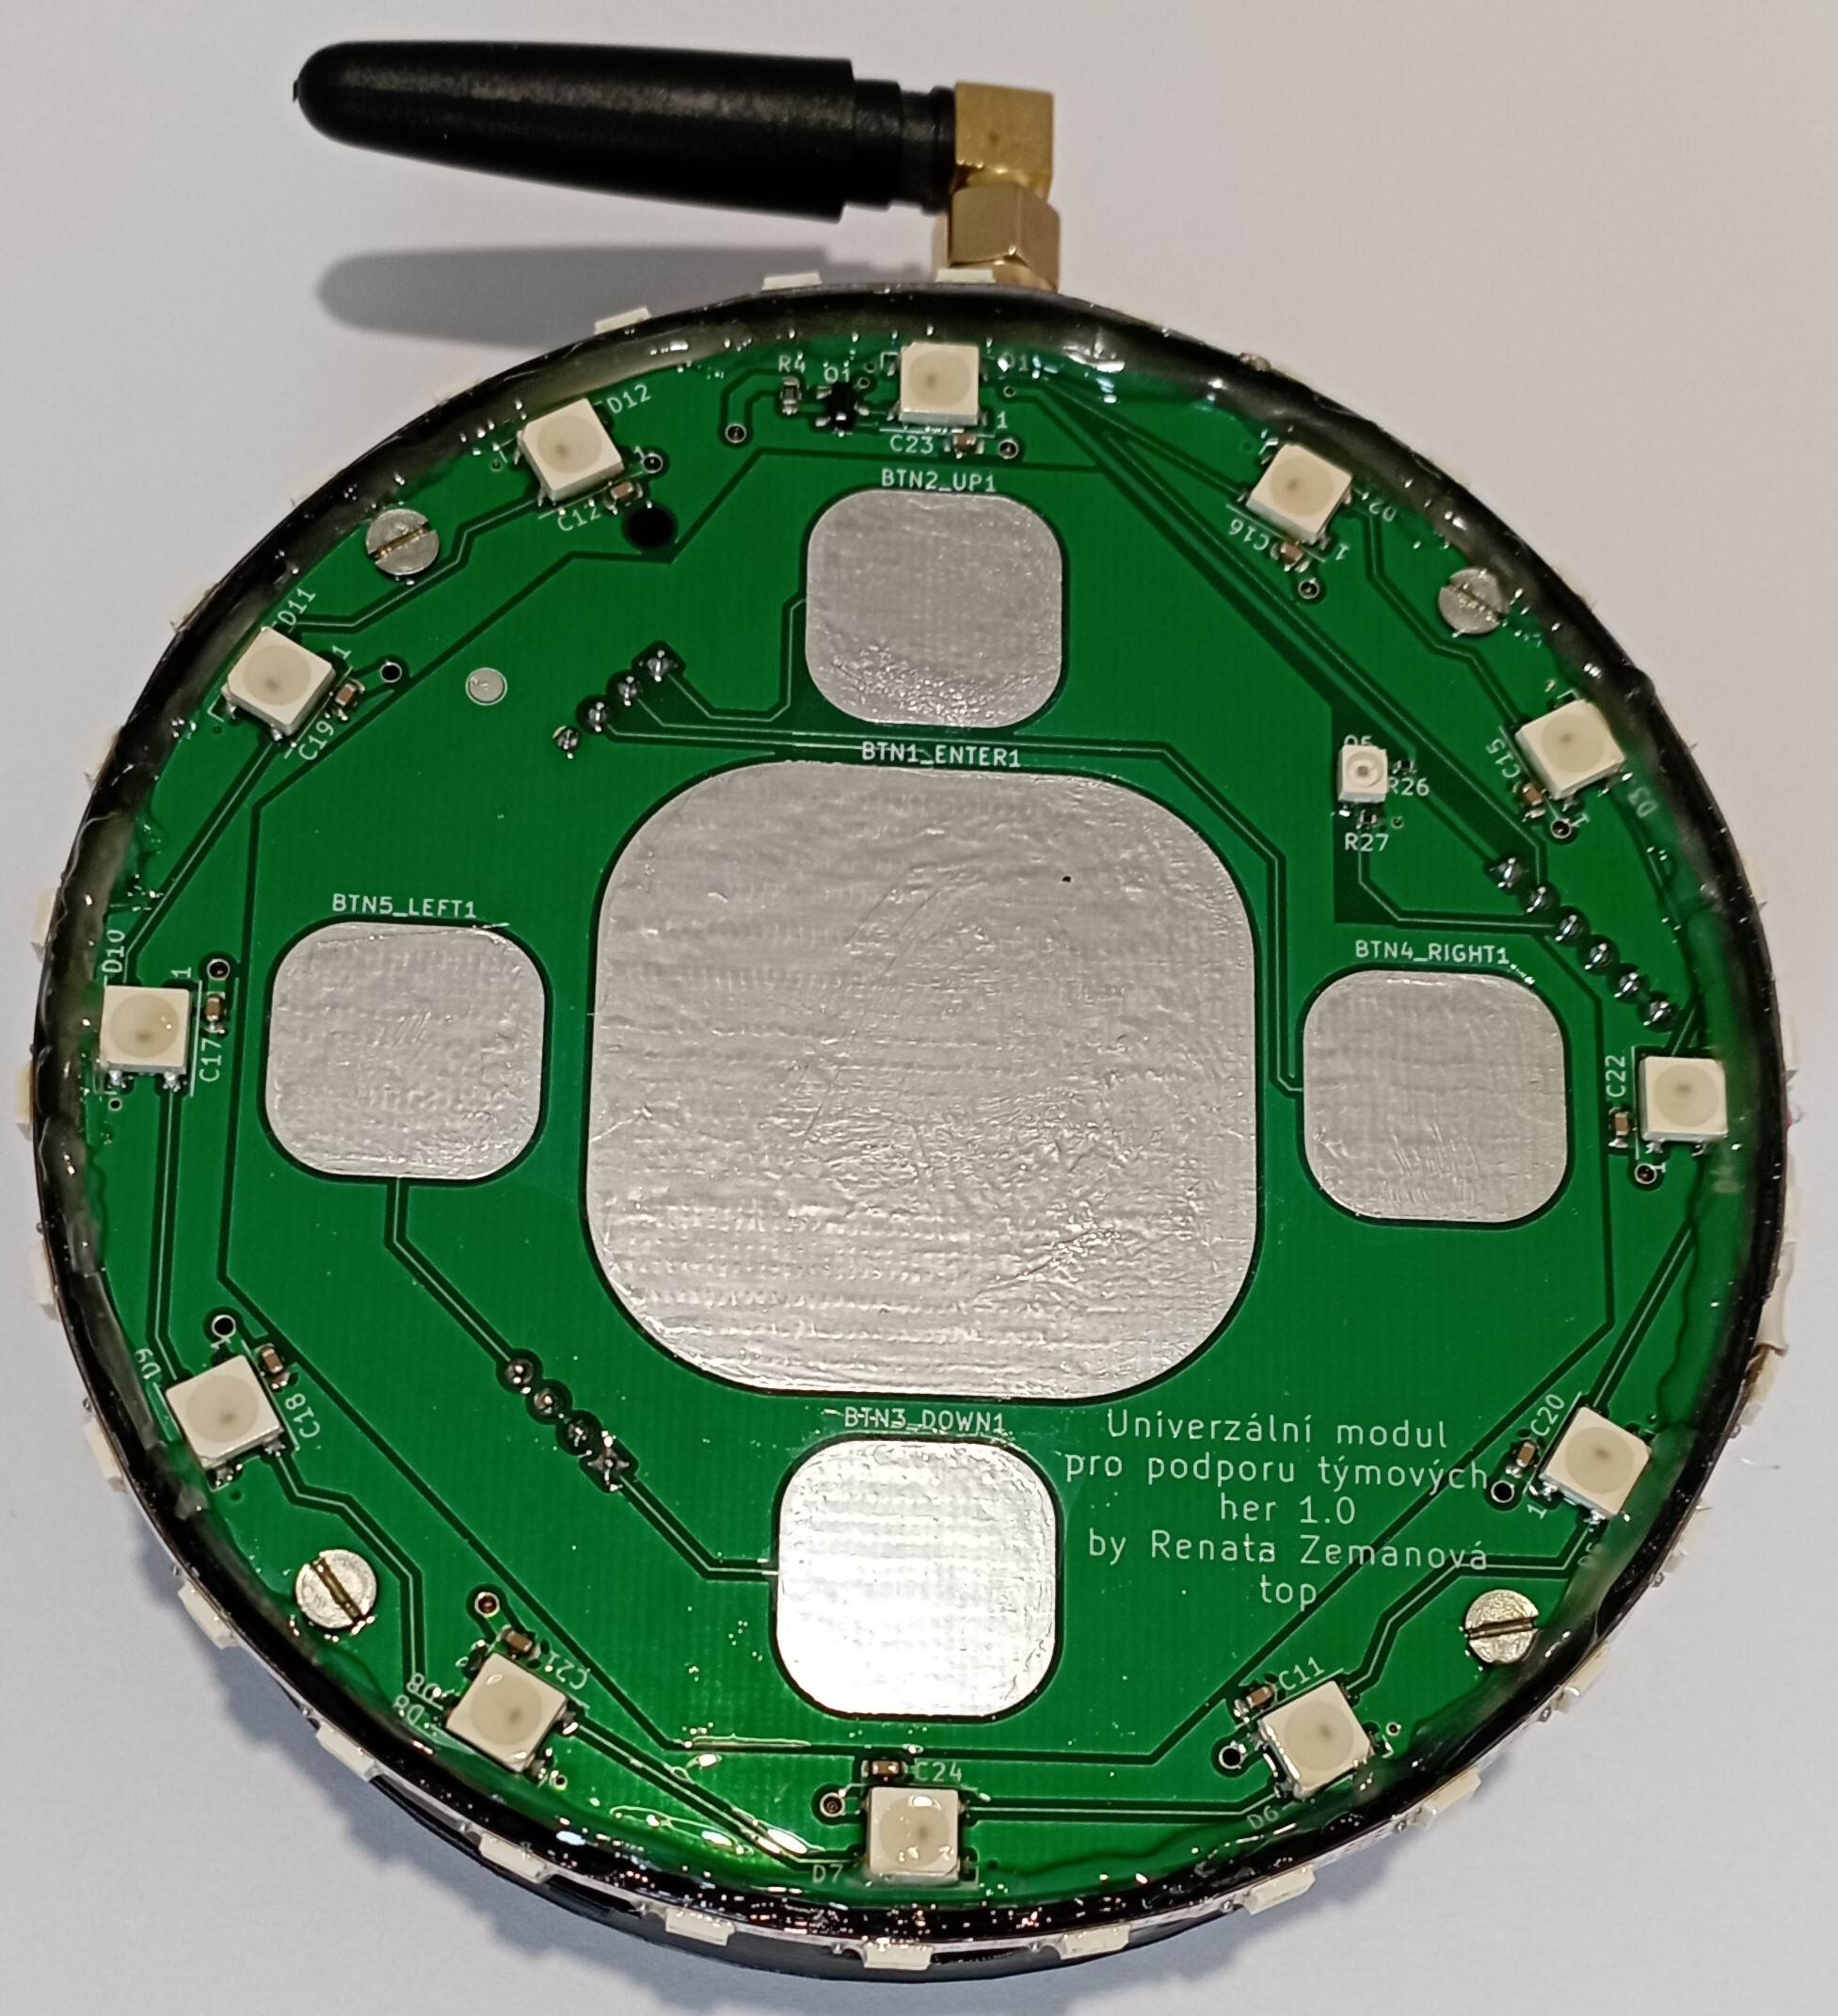
\includegraphics[width=0.65\columnwidth]{obrazky/v_krabicce.jpg}
				\end{figure}
			\end{column}
		\end{columns}	
	\end{center}
\end{frame}

\begin{frame} 
	\frametitle{Otázky oponenta}
	\emph{Jak je řešená ochrana proti podbití? Jaký bude mít vliv na další vybíjení baterie napěťový dělič mezi R1 a R7 a rezistor R12 s diodou D16?}
	\begin{itemize}
		\item Není řešeno hardwarově
		\item Softwarové vypínání napětí LED, LoRa modulu, zvyšovače napětí LT1930 a~převodníku pro kapacitní tlačítka AT42QT1070 
		\item Přechod mikrokontroléru nebo LoRa modulu do režimu spánku 
		\item MCU - 130 $\mu$A, powerLED - 3,3 mA, rezistorový dělič - 58 $\mu$A 
	\end{itemize}

	\begin{figure}
		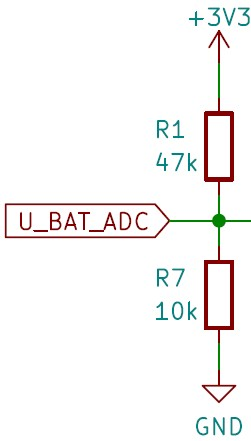
\includegraphics[width=0.13\columnwidth]{obrazky/dotaz_delic.jpg}
		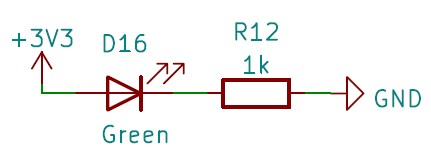
\includegraphics[width=0.28\columnwidth]{obrazky/dotaz_power_LED.jpg}
	\end{figure}
	
\end{frame}

\begin{frame} 
	\frametitle{Otázky oponenta}
	\emph{Jaká je celková spotřeba zařízení v běžném provozu a jak dlouho je baterie schopná v tomhle stavu modul napájet?}
	\begin{itemize}
		\item Kapacita baterie - 1800 mAh
		\item Herní mód Odpočítávání - 200 mA 
		\item 9 hodin provozu 
	\end{itemize}
\end{frame}

\end{document}
